\documentclass[11pt,a4paper]{article}
\usepackage[utf8]{inputenc}
\usepackage[margin=1in]{geometry}
\usepackage{amsmath,amssymb,amsthm,mathtools}
\usepackage{booktabs}
\usepackage{array}
\usepackage{graphicx}
\usepackage{float}
\usepackage{caption}
\usepackage[hidelinks]{hyperref}
\usepackage{natbib}
\bibliographystyle{plainnat}
\usepackage[expansion=false]{microtype}
\usepackage{setspace}
\onehalfspacing
\setlength{\emergencystretch}{3em}

\theoremstyle{plain}
\newtheorem{proposition}{Proposition}
\newtheorem{corollary}[proposition]{Corollary}
\newtheorem{lemma}[proposition]{Lemma}
\theoremstyle{definition}
\newtheorem{definition}{Definition}
\newtheorem{remark}{Remark}
\newtheorem{assumption}{Assumption}

\DeclareMathOperator*{\argmax}{arg\,max}
\newcommand{\Prob}{\mathbb{P}}
\newcommand{\E}{\mathbb{E}}
\newcommand{\ind}[1]{\mathbf{1}\{#1\}}


\title{\bfseries Online appendix: case studies and a neural procedure for proposing settings\\
\large to ``Governing privacy risk across repeated statistical releases''}

\author{Ronald Rethabile Malamule Mahomane\thanks{Corresponding author:
\texttt{ron@basisenergygroup.com}. This is an author manuscript, not a BIS or IFC publication.}\\
\small Department of Computing, Mathematical and Statistical Sciences,
University of Namibia, Windhoek\\
\small School of Pathology, Faculty of Health Sciences,
University of the Witwatersrand, Johannesburg\\
\small Basis Energy, Victoria, Australia}

\date{Author manuscript: September 2026}

\begin{document}
\maketitle

\noindent This online appendix goes with the author manuscript ``Governing privacy risk across repeated statistical releases: probability models, programme tolerances and accountable decisions''. It holds material that the main text refers to but does not need: case studies from other data products, and a neural procedure for proposing candidate settings, with its variant SENTRY-R. Nothing here enters the results of the main text. Where this appendix refers to the main text it names the section or result rather than giving a number. Every numerical table here is produced by the packaged pipeline in the companion repository.

\section{Case studies from other data products}\label{sec:cases}

The cases below are not pooled into one empirical estimate. They concern
different data products, adversaries and harm classes, and the published evidence
does not support a common denominator. Each case identifies which component of
the proposed decision record would have made the public claim more precise.
Table \ref{tab:cases} records that mapping. Each row reads from left to right:
what was released and how it was attacked, the object of the framework that
describes the attack, and what the case teaches about the decision record. The
last column carries the point of the table: in each case the public claim lacked
a part of the record, such as a declared adversary, a programme guarantee, a
decision owner or a stated residual risk. The first row is the credit register
of the main text (the section on a granular credit register), treated there with measurements; the
other four are not central bank cases and are described here without new
measurements.

\begin{table}[htbp]
\centering
\caption{Case studies mapped to the framework}
\label{tab:cases}
\small
\begin{tabular}{p{2.7cm}p{3.0cm}p{3.1cm}p{4.1cm}}
\toprule
Case & Release and attack & Mathematical object & Governance lesson \\
\midrule
Granular credit register & Loan-level file, aggregates and monthly revisions &
Identification, predictive value of an alleged relationship, attribute and
residual disclosure, differencing & One lever does not govern five risks; each
needs its own target set and tolerance. \\
Netflix Prize & Sparse ratings linked to outside ratings & Posterior linkage
$p_{tj}$ and pooled auxiliary information & ``Anonymous'' identifiers do not
define an adversary or bound posterior success. \\
US Census 2020 & Published tabulations and database reconstruction & Programme
composition and formal privacy accounting & Repeated exact statistics require
a programme guarantee, not isolated marginal checks. \\
England and Wales Census 2021 & Tables protected by record swapping and cell-key
perturbation & Mechanism risk--utility frontier & Operational protection must be
paired with an explicit scenario, uncertainty statement and decision owner. \\
HIPAA de-identification & Safe Harbor or Expert Determination & Rule-based versus
scenario-based threshold & A legal route is not itself a numerical probability;
Expert Determination makes assumptions and residual risk reviewable. \\
\bottomrule
\end{tabular}
\end{table}

\subsection{Sparse behavioural data: the Netflix Prize}

The Netflix Prize data replaced direct identifiers with pseudonymous user
numbers, but the released rating vectors were high-dimensional and sparse.
\citet{narayanan2008} showed that a small amount of auxiliary rating information
could link records across datasets. In the notation of the main text (the unified linkage experiment), the released identifier was irrelevant to the attack:
$Z_t$ contained a few ratings and approximate dates, $L_{tj}$ measured their
agreement with candidate records, and the largest posterior in
the maximum-posterior rule of the main text determined the match. The case therefore illustrates the
failure of exchangeability, not merely the presence of sample uniques.

The defensible retrospective test is not whether the file was anonymised. It is:
for a prespecified distribution of auxiliary ratings and date error, what is the
distribution of $\max_j p_{tj}$ across targets, and what simultaneous upper bound
lies below the owned tolerance? A modern replication should vary the number of
auxiliary ratings, their popularity, the date tolerance and the abstention
threshold. Those variables define a family of attacks; choosing only an easy one
after seeing the outcome would not validate the release.

\subsection{Repeated official statistics: the 2020 US Census}

The US Census Bureau adopted a disclosure avoidance system built on differential
privacy \citep{abowd2018} after demonstrating that many published tabulations can support database
reconstruction \citep{garfinkel2019,abowd2022,abowd2023}. This is the
institutional case closest to the proposition of the main text that marginal risks do not bound pooled risk. The threat does not
arise because one table has a large marginal linkage risk. It arises because many
accurate, overlapping constraints describe the same underlying population.

The framework makes two distinctions. First, reconstruction, membership inference
and correct named-person linkage are different events and must not be reported
under one risk label. Second, a formal privacy accountant governs the programme
mechanism, whereas $\sum_i R_i$ governs only a union of declared single-release
attacks. The policy debate over accuracy remains a risk--utility choice, but the
protection claim and its unit of composition are now explicit. The appropriate
empirical study would compare redistricting, small-area and demographic estimands
under alternative privacy-loss budgets, then report subgroup-specific utility
losses beside the programme guarantee. \citet{ruggles2019} set out the costs of
the change for social and economic research, and \citet{kenny2021} find that the
new system biases the population of mixed precincts used in redistricting.

\subsection{Layered operational protection: Census 2021 in England and Wales}

The Office for National Statistics describes protection of Census 2021 outputs
through record swapping and the cell-key method, together with checks against
disclosure in tables \citep{ons2022}. This is not evidence that the release has a
universal linkage probability, nor need it be. It is evidence of a layered
mechanism $M_\theta$ whose tuning changes both tabular accuracy and the
information available to an intruder.

For governance, what is missing is a declared attack experiment. An evaluation
could draw targets from separately stated population groups, expose the attacker
to realistic public registers, reproduce the cell-key and swapping randomness,
and calculate $\overline{R}_{1-\alpha}$ for each protected group. The mechanism
parameters, the seeds policy, the table family and the expiry date would then be
part of the governance threshold $G$ defined in the main text. That turns a process description into a
reproducible release decision, without implying that the mechanism offers
differential privacy unless it does.

\subsection{Health data: HIPAA Safe Harbor and Expert Determination}

US health-data guidance recognises two routes for de-identification: removal of
specified identifiers under Safe Harbor, and Expert Determination that the risk
of identification is very small, using generally accepted statistical and
scientific principles \citep{hhs2012}. The contrast maps directly to this paper.
Safe Harbor constrains the released variables; Expert Determination is a
scenario-conditioned judgement about residual risk. Neither phrase alone fixes
$T$, $a$, $h$, $\tau$ or $\alpha$.

A complete determination would therefore file the population and target set, the
accessible auxiliary sources, the linkage rule, the harm class, the estimate, the
uncertainty bound and the review horizon. Where data are released repeatedly to
the same recipient, the determination must count the accumulated products as part
of what the adversary holds. This does not replace legal judgement. It makes the
empirical premises of that judgement capable of expiry, challenge and
replication.

\subsection{A common case-study protocol}

Across the five settings, a comparable prospective study has seven steps:

\begin{enumerate}
\item freeze the release mechanism, and define neighbouring or alternative
confidential states where a formal guarantee is claimed;
\item specify the target population, the auxiliary information and the abstention
rule;
\item separate linkage, membership, attribute and reconstruction success events;
\item simulate or execute attacks with the mechanism randomness and the shared
data dependencies preserved;
\item estimate target and subgroup risks with simultaneous uncertainty bounds;
\item measure utility on prespecified authorised analyses, including subgroup
error rather than only an aggregate score; and
\item assess the complete release programme, then file the governed tuple $G$.
\end{enumerate}

The resulting studies would be comparable in design while keeping different
numerical scales where the estimands genuinely differ.

\section{An audited margin vector with a neural proposal model}\label{sec:neural}

A release decision needs a measured quantity, not a score. For a proposed mechanism
$\theta$, let $j=(a,h,g,v)$ index an adversary, harm class, target group and
release vintage, including a separate index for an attacker pooling vintages.
The finite, declared index set is $\mathcal J$, of cardinality $n$. A scenario
$j$ fixes the target sampling frame, attack algorithm, access to auxiliary
information, release programme and binary definition of success. Conditional
on a fixed proposed release and these specifications, let $P_{\theta j}$ be
the law of one fresh attack experiment and define the actual risk
$r_j(\theta)=\E_{P_{\theta j}}S_j$, where $S_j\in\{0,1\}$ records success.
The tolerance $\tau_j\in(0,1)$ is fixed before the final audit. A population
average and a particular target require distinct scenario definitions.
A neural score does not supply this quantity. We call the vector of
independently audited margins the \emph{audited margin vector}, and its
smallest entry the \emph{minimum audited margin}:
\begin{equation}
 {\bf z}(\theta)=\left(1-\frac{\overline r_j(\theta)}{\tau_j}
                  \right)_{j\in\mathcal J}\in\mathbb R^n,
 \qquad T(\theta)=\min_{j\in\mathcal J}z_j(\theta).
 \label{eq:trust-position}
\end{equation}
Here $\overline r_j$ is a simultaneous upper confidence bound, with its sampling
unit and adversary written into the assessment. A nonnegative $T$ means every
declared coordinate passes. The complete vector must accompany the scalar: the
minimum alone conceals which group or programme attack constrains the release.
Utility $U(\theta)$ is kept as a separate coordinate, since a release can have
large audited margins while carrying little public value. Missing or
unaudited coordinates receive $\overline r_j=1$ and therefore fail whenever
$\tau_j<1$. Each assessment thus starts with no inherited claim of safety:
collect independent evidence, tighten the bounds, improve the mechanism, and
recertify. It does not promise that evidence will rescue an unsafe release.

Figure \ref{fig:trust-vector} depicts the coordinatewise decision. Each entry
is a separately audited margin, and one negative entry forces the minimum
below zero even if the other coordinates pass.
\begin{figure}[H]
\centering
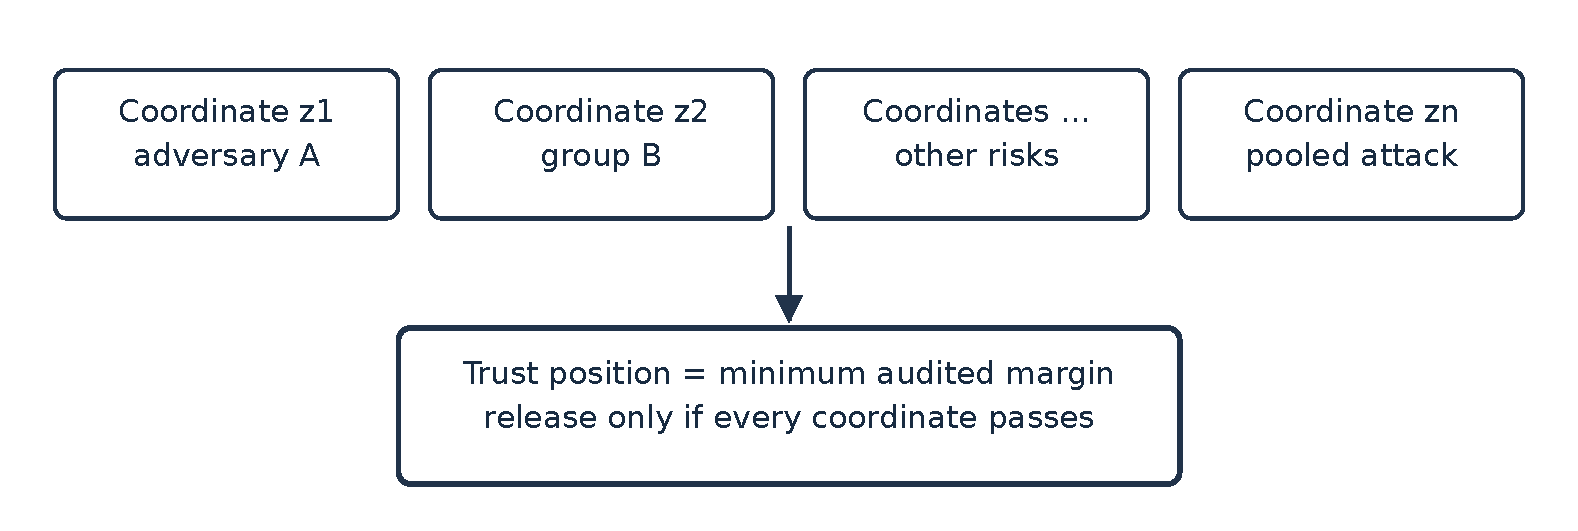
\includegraphics[width=.94\linewidth]{diagrams/trust_vector.pdf}
\caption{The $n$-dimensional trust position uses independently bounded risk coordinates $z_j=1-\overline r_j/\tau_j$. The labels illustrate declared coordinates, not numerical results.}
\label{fig:trust-vector}
\end{figure}


\subsection{The neural model and what its output means}

Encode a proposed release and its environment as $x(\theta)\in\mathbb R^d$:
mechanism parameters, sample fraction, key entropy and sparsity, auxiliary
information quality, number and overlap of prior releases, access controls,
population shifts and target-group indicators. All features must be available
\emph{before} certification and their provenance recorded. A transparent
baseline is a regularised logistic model; our nonlinear proposal model is
\begin{align}
 H_0&=x, &H_{\ell+1}&=\rho(H_\ell W_\ell+b_\ell),\quad 0\leq\ell<L,\\
 \widehat{\boldsymbol r}_{\phi}(x)
   &=\sigma(H_LW_{\rm out}+b_{\rm out})\in(0,1)^n,
 &\mathcal L(\phi)&=-\sum_{i,j}w_{ij}
  [y_{ij}\log\widehat r_{ij}+(1-y_{ij})\log(1-\widehat r_{ij})].
 \label{eq:neural-risk}
\end{align}
The \texttt{neural\_trust} module fixes $L=1$; \texttt{sentry\_r} makes $L$
configurable.
The label $y_{ij}$ is the \emph{observed success of an attack} on a separate
scenario draw, with a zero label for a failed or abstaining attack as specified
in the threat model. Unevaluated pairs have $w_{ij}=0$; repeated attacks sharing
one auxiliary file are clustered by file rather than treated as independent.
The sigmoid outputs are predicted attack frequencies, not audited margins or
probabilities that a release is safe, and no ordering of them across harm classes is implied.
Train on past mechanism--adversary scenarios, hold out whole populations,
release programmes and vintages, and keep the final audit draws out of all
training, tuning, calibration and feature selection. Compare log loss, Brier
score and reliability diagrams with the logistic and frequency baselines, both
overall and by group \citep{guo2017}. A calibration plot is a diagnostic, never a certificate
for the highest-risk individual.

The neural model proposes a \emph{finite} shortlist $\Theta_0$: it ranks
candidates by their largest predicted risk-to-tolerance ratio; utility enters
only the final choice among certified candidates. For each candidate and $j$, run $B_{\theta
j}$ fresh, conditionally identically distributed Bernoulli attacks and count
$K_{\theta j}$ successes. Fix the sample sizes before observing final outcomes.
With $M=|\Theta_0|n$ prespecified inspected coordinates,
define the exact one-sided bound
\begin{equation}
 \overline r_{\theta j}=
 \begin{cases}
 1,&K_{\theta j}=B_{\theta j},\\
 F^{-1}_{\mathrm{Beta}(K_{\theta j}+1,\,B_{\theta j}-K_{\theta j})}
      (1-\alpha/M),&K_{\theta j}<B_{\theta j}.
 \end{cases}\label{eq:neural-audit}
\end{equation}
Certification uses \eqref{eq:trust-position} and \eqref{eq:neural-audit}, never
the neural output. The final choice may maximise $U$ among certified candidates,
provided the shortlist was fixed without looking at these final audit draws.

Figure \ref{fig:neural-workflow} makes the separation between development
and final evidence explicit. The arrows into the final gate carry audit
bounds and tolerances; the network contributes only the fixed shortlist.
\begin{figure}[H]
\centering
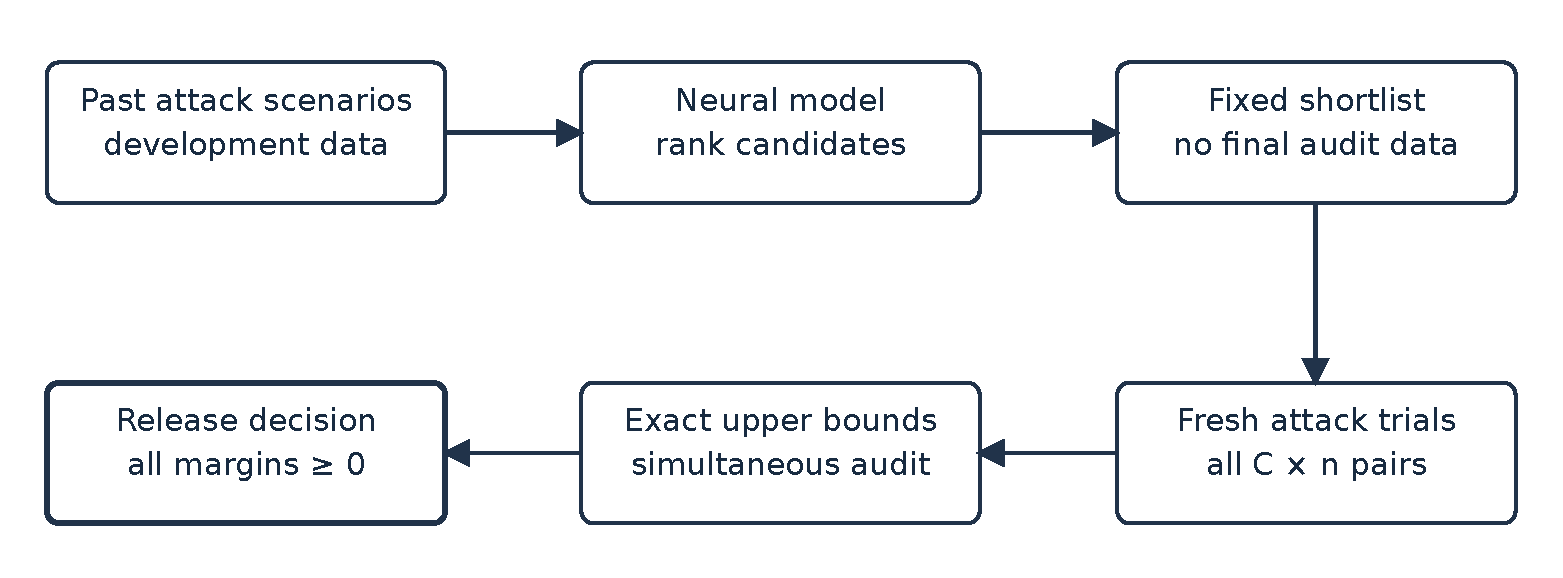
\includegraphics[width=.94\linewidth]{diagrams/neural_workflow.pdf}
\caption{The neural network ranks candidates; independent attack trials and exact simultaneous upper bounds decide. $C=|\Theta_0|$ and $n$ is the number of risk coordinates.}
\label{fig:neural-workflow}
\end{figure}


\begin{proposition}[Selection-safe finite-family certification]\label{prop:neural-gate}
Condition on development information $\mathcal D$ and its resulting finite
shortlist, candidate releases, scenarios and sample sizes. Suppose each final
audit count is $\mathrm{Binom}(B_{\theta j},r_j(\theta))$ conditional on
$\mathcal D$; auxiliary information sampled afresh is included in this
experiment, whereas fixed auxiliary information is conditioned upon. Then
with probability at
least $1-\alpha$, simultaneously for every inspected pair,
$r_j(\theta)\leq\overline r_{\theta j}$. Consequently the rule selecting any
candidate with $T(\theta)\geq0$ has probability at most $\alpha$ of certifying
a candidate whose risk exceeds a declared tolerance in any coordinate.
\end{proposition}
\begin{proof}
For one pair the event that the exact upper bound falls below the true risk
has probability at most $\alpha/M$ by inversion of the binomial lower-tail
test (Appendix \ref{app:neural}). A union bound over the $M$ pairs gives the
simultaneous statement, without requiring independence between pairs. On this
event every certified candidate satisfies $r_j(\theta)\leq\tau_j$ for all
$j$, regardless of which certified candidate the final rule selects.
Taking expectation over $\mathcal D$ gives the unconditional guarantee.
\end{proof}

If the release, attack, shortlist or group definitions change in response to
final outcomes, the conditional argument no longer applies. Freeze and restart
with untouched audit draws, or replace the fixed-sample bound by the anytime
procedure of the main text (the section on adaptive attacks and anytime-valid certification) with an explicit multiplicity
allocation. Binomial sampling covers attack-draw variability conditional on a
fixed population and mechanism. It does not cover uncertain input data, unknown
auxiliary sources, a stronger future attacker or distribution shift. Those are
separate scenario coordinates or require a stated outer uncertainty analysis.

\subsection{What changes as the dimension grows}

The number $d$ of input features and the number $n$ of risk coordinates are
different. For widths $q_0=d,q_1,\ldots,q_L,q_{L+1}=n$, a dense forward pass
costs $O(\sum_{\ell=0}^{L}q_\ell q_{\ell+1})$ operations per scenario and
stores $O(\sum q_\ell q_{\ell+1})$ parameters; a training epoch multiplies
the cost by the number of labelled scenarios. Sparse embeddings or shared
encoders can reduce cost when many groups share structure, but cannot supply
evidence in an unseen group. A full final audit over $C$ candidates and $n$
coordinates uses $Cn$ confidence bounds and, at zero observed successes in
every coordinate, needs at least
\begin{equation}
 B\geq\left\lceil\frac{\log(\alpha/(Cn))}{\log(1-\tau_{
 \min})}\right\rceil\label{eq:neural-budget}
\end{equation}
independent trials per coordinate to certify a common minimum tolerance
$\tau_{\min}$. This is necessary and sufficient when that coordinate has
zero successes; with successes, more trials can be needed. Thus computational
amortisation by a network
does not erase the statistical cost of many simultaneous guarantees.
For an $L$-Lipschitz risk function on $[0,1]^d$, even a direct grid at
accuracy $\epsilon$ uses order $(L/\epsilon)^d$ cells. Without such
regularity, finite observations alone cannot guarantee uniform pointwise
accuracy. Report learning curves against both $d$
and $n$; do not describe merely adding hidden units as solving this problem.

For stress testing, if the full law $Q_{\theta j}$ of the deployed attack
experiment is known to satisfy
$\mathrm{TV}(P_{\theta j},Q_{\theta j})\leq\delta_j$,
bounded attack success gives
$r_{Q_{\theta j}}(\theta)\leq r_{P_{\theta j}}(\theta)+\delta_j$.
A declared and justified
bound can therefore replace $\overline r_j$ by
$\min(1,\overline r_j+\delta_j)$. Estimating $\delta_j$ from a neural
embedding alone does not justify that guarantee. Out-of-scope feature values,
new linkage data and an unbounded shift require refusal and a new assessment.

The testable methodological contribution is the combination of an audited
margin vector, a neural search model, and an independent simultaneous audit
under adaptive choice of the final candidate. Neural prediction, binomial
bounds and neural calibration individually have extensive precedents
\citep{bates2021,guo2017}; the
claim here is about their stated division of labour for a release programme,
not an untested claim of superior empirical performance. The accompanying
\texttt{privacy\_risk.neural\_trust} module includes a seeded synthetic demonstration of the search
and audit interface. It cannot validate the existing tables in this paper.
An empirical extension must preregister targets and populations, compare the
network with the logistic and frequency baselines at fixed audit budgets,
report selective utility and worst-group failures, and rerun every pooled
attack on held-out real programmes.

\section{SENTRY-R: scenario-enriched neural triage for release review}\label{sec:sentry}

We name the implementable extension \emph{SENTRY-R}, shorthand for
scenario-enriched neural triage for release review. This names the specified
workflow, not a claim that its
components are individually new or that a fitted network has improved real
release decisions. Its separation of three data streams is central:
\emph{untrusted scenario proposals}, \emph{measured development attacks}, and
\emph{untouched final audits}. The implementation supports any finite input
dimension $d$ and any finite number $n$ of declared risk coordinates. A deeper
network predicts attack frequencies for search; it does not certify a release.

\subsection{LLM-assisted scenario expansion and evidence provenance}

Let $\mathcal F_t$ denote the information available before development round
$t$, including past mechanisms, validated scenario specifications and measured
attacks. A language model proposes descriptions and numeric scenario features
$Q_t=G_t(\mathcal F_t,\xi_t)$. A deterministic validator checks the predeclared
feature names and bounds and the scenario identifier. The calling code, not
the language model, writes the source metadata: the model name and the
SHA-256 hash of the exact prompt. The validator does
not treat free-form text or a language-model risk estimate as an observed
success. A separate attack evaluator then draws $Z_{ti}$ under the accepted
scenario and records $K_{tj}=\sum_{i=1}^{B_{tj}}s_j(Z_{ti})$, together with
its experiment identifier and sampling unit. The retraining history grows by
\begin{equation}
 \mathcal F_{t+1}=\mathcal F_t\vee\sigma\!\left(Q_t,\operatorname{valid}(Q_t),
 \{K_{tj},B_{tj},\operatorname{provenance}_{tj}\}_{j\in\mathcal J}\right).
 \label{eq:sentry-filtration}
\end{equation}
The language model can change which \emph{development} experiment is run next;
it does not directly change a network weight or label. Source identifiers,
scenario hashes and an explicit partition label make the update inspectable.
Treating repeated targets or auxiliary files as independent Bernoulli trials
would break the specified sampling model. Human review is still required to
establish whether a proposed adversary, harm definition and auxiliary source
are plausible and permissible.

Let $\mathcal D=\mathcal F_{t_*}$ be all such development information at a
chosen stopping time $t_*$, including model weights and hyperparameter
selection. A separate validation set holds out entire release programmes;
final audit draws are excluded from $\mathcal D$. Conditional on $\mathcal D$,
freeze the coordinate definitions, policy tolerances, $C$ shortlisted
candidates, the family error $\alpha$ and the planned sample sizes
$B_{\theta j}$. The implementation writes all of these, with a named
tolerance owner, an expiry date and every development evidence identifier,
into one hashed freeze record. The final audit reads $\alpha$ from that
record and refuses to run if the record has changed, if the expiry date has
passed, if any trial count differs from the plan, or if an audit evidence
identifier was used in development. An optional append-only ledger refuses a
second audit of the same freeze. These checks bind an audit to its freeze.
On their own they do not prove the order of events, since the freeze hash has
no key or trusted time stamp. An optional keyed ledger records a stronger
local history: each instrumented stage, from the language model's proposal through
review, measurement, training and freeze to the audit, is appended to one
hash-chained file, each entry signed with HMAC-SHA256 under a key the operator
holds, and an entry is refused unless the entries it depends on are already on
the chain. The same ledger holds each programme's error budget and debits
every recorded audit's $\alpha$ against it. New measurement entries also commit
the full measured row, so changed features or counts are refused when recording
a training artifact. These checks apply when provenance and proposal lineage
are retained. Base evidence, reviewer identities and evaluator authenticity
remain caller-controlled, and an operator can omit provenance or relabel data.
The audit debit occurs after outcomes are supplied; it does not prevent an
operator from obtaining or discarding outcomes outside the recorded path. A
service must reserve budget before draws, preserve every attempt and anchor
chain heads outside the operator's control. A key holder can otherwise rewrite
the file. Under the stated statistical assumptions, Proposition
\ref{prop:neural-gate} guarantee then applies even if the \emph{development}
sequence used an LLM adaptively, provided the conditional binomial model for
the untouched final draws holds. A final audit reused as development data, or
an LLM proposal generated from its outcomes, invalidates that conditioning.
Figure \ref{fig:sentry-loop} shows the implemented boundary. It reads from left
to right and then down. A scenario proposed by a language model passes a fixed
schema and a named review, and it can add a scenario but never an outcome. Only
counted development attacks train the deep proposal model, whose ranking fixes a
shortlist of candidate settings. Only the fresh final audit, with simultaneous
bounds over every coordinate, reaches the release decision. The note under the
first box states the rule the figure is there to show: proposal text never
supplies a training label or a release certificate.
\begin{figure}[tbp]
\centering
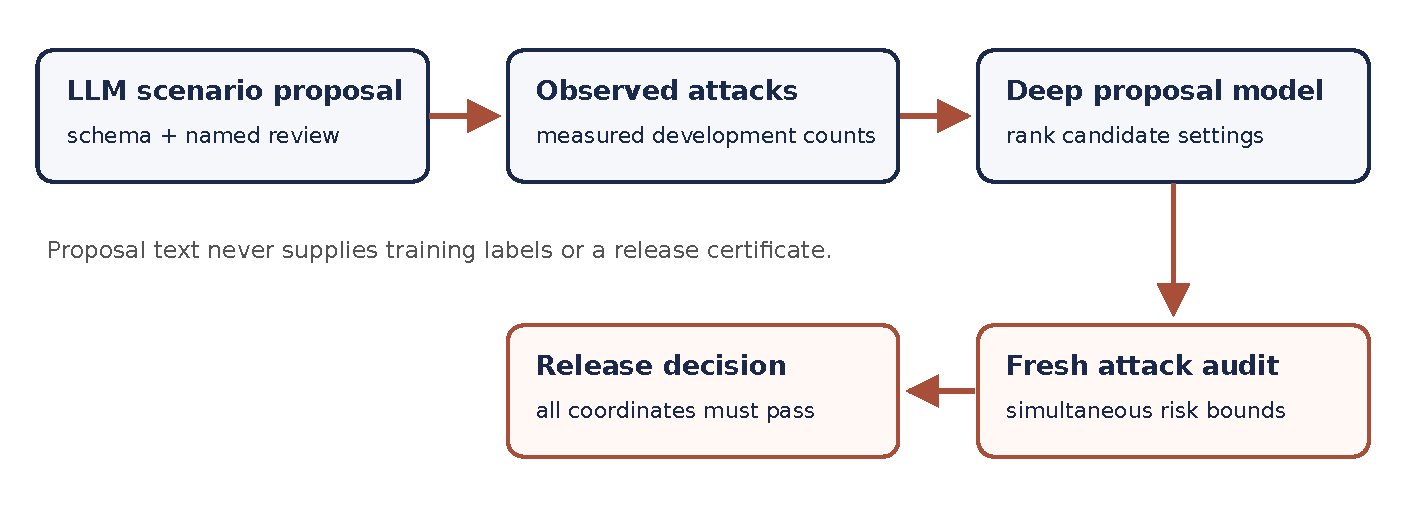
\includegraphics[width=0.95\linewidth]{diagrams/sentry_r_loop.pdf}
\caption{SENTRY-R development and decision boundary. The LLM's scenario proposal is checked against a fixed schema; only measured development attacks enter the deep model. Its ranking freezes a shortlist before a fresh, independent final audit.}
\label{fig:sentry-loop}
\end{figure}


\subsection{A deep model trained on counted attack outcomes}

The \texttt{privacy\_risk.sentry\_r} module provides a depth-$L$ fully connected
ReLU model with common width $q$, including the depth-zero logistic baseline.
Training features $x_i\in\mathbb R^d$ are standardised using \emph{training}
means and scales only. With $h_i^0=x_i$, for $\ell=0,\ldots,L-1$ define
\begin{equation}
 h_i^{\ell+1}=\rho(h_i^\ell W_\ell+b_\ell),\quad
 a_{ij}=\left(h_i^L W_{\mathrm o}+b_{\mathrm o}\right)_j,\quad
 p_{ij}=\sigma(a_{ij}),\quad \rho(z)=\max\{0,z\}.
 \label{eq:sentry-deep}
\end{equation}
For each observed development pair $(i,j)$ let $K_{ij}\in\{0,\ldots,B_{ij}\}$
be the count of successes in $B_{ij}\geq1$ trials. The implementation
minimises the binomial negative log likelihood, without its constant
combinatorial term, and a ridge term:
\begin{equation}
 \mathcal L(\phi)= -\frac{1}{B_\bullet}\sum_{i,j}
 \left[K_{ij}\log p_{ij}+(B_{ij}-K_{ij})\log(1-p_{ij})\right]
 +\frac{\lambda}{2}\sum_{\ell=0}^{L}\|W_\ell\|_F^2,
 \quad B_\bullet=\sum_{i,j}B_{ij}.
 \label{eq:sentry-count-loss}
\end{equation}
Here $W_L=W_{\rm o}$; a weight attached to trial count is appropriate only if
the count's sampling design was fixed without peeking at those outcomes. To
see exactly what is learned, assume $K\mid x,B\sim\mathrm{Binom}(B,\pi_j(x))$
with $B$ determined before outcomes. For a fixed $x,B$, the expected
unregularised loss minus its value at $p=\pi_j(x)$ is
\begin{equation}
 \frac{B}{B_\bullet}\,D_{\mathrm{KL}}
 \left(\mathrm{Bern}(\pi_j(x))\,\|\,\mathrm{Bern}(p)\right)\geq0.
 \label{eq:sentry-proper}
\end{equation}
Thus the ideal unrestricted conditional predictor is the attack success
frequency $\pi_j(x)$ on the \emph{development} distribution; finite data,
regularisation, optimiser error and population shift prevent equality in an
actual trained model. No neural output is a confidence limit on an individual
or a new population.

The model is fitted by backpropagation. With $P=(p_{ij})$, $K=(K_{ij})$ and
$B=(B_{ij})$, the output-logit derivative is $(B\odot P-K)/B_\bullet$, and the
hidden-layer gradients follow by the chain rule in the usual way
\citep[ch.~6]{goodfellow2016}. The package includes a finite-difference check of
the derivatives.

\subsection{Training, scale and falsification}

The network uses seeded mini-batches, Adam, gradient clipping and early
stopping on a separate held-out programme. Depth zero is trained on the same
counted outcomes as a logistic baseline. For $N$ development rows and $E$
epochs, the dense leading arithmetic order is
$O\{EN[dq+(L-1)q^2+qn]\}$ for $L\geq1$, with
$O\{dq+(L-1)q^2+qn\}$ weights; the logistic case has $O(ENdn)$
arithmetic. This is a computational scaling statement, not a statistical
sample-size promise. The final $Cn$ confidence bounds and independent attack
trials remain necessary whatever the prediction speed. Unknown groups and
out-of-domain features trigger a new assessment rather than an extrapolated
certificate.

A valid empirical evaluation must compare deep and logistic rankings at fixed
shortlist sizes and audit budgets on held-out \emph{real} programmes; report
log loss, Brier score, worst-group calibration, selected utility and false
gates; repeat pooled-vintage attacks; and show uncertainty across programmes.
This package currently provides a seeded synthetic end-to-end demonstration,
not such an evaluation. Table \ref{tab:sentry-synthetic} is regenerated by
\texttt{scripts/sentry\_r\_benchmark.py}. For each of ten seeds it draws
three disjoint programmes from one toy law: 320 training rows, 100 rows used
only for early stopping, and 2,000 test rows used only for the reported loss.
Both models train until 150 epochs pass without improvement, and no best
epoch reaches the cap. Trained to convergence, the logistic model has a
slightly lower test log loss than the three-layer model in all ten
replicates. The mean paired gap is smaller than the spread of either model
across replicates. The table shows that the pipeline runs, not that depth
helps. The test programmes come from the same law and feature range as the
training data, so they do not test shift.
\begin{table}[H]
\centering
\small
\caption{Synthetic SENTRY-R comparison over 10 seeded replicates of the toy law. Each replicate draws 320 training rows, 100 rows used only for early stopping (patience 150 epochs, cap 6000) and 2000 test rows used only for the reported losses. Entries are mean (standard deviation) across replicates; smaller is better. The last row is the paired deep-minus-logistic test log loss (range 0.0004 to 0.0050; deep lower in 0 of 10). These are not results on real release programmes.}
\label{tab:sentry-synthetic}
\begin{tabular}{lrrr}
\toprule
Proposal model & Test log loss & Test Brier score & Best epoch (range) \\
\midrule
Logistic & 0.2556 (0.0043) & 0.0727 (0.0017) & 404--898 \\
Three-layer ReLU & 0.2576 (0.0047) & 0.0735 (0.0018) & 79--402 \\
\midrule
Deep minus logistic & 0.0020 (0.0014) & & \\
\bottomrule
\end{tabular}
\end{table}


\section{Mathematical details for the audited margin vector}\label{app:neural}

\paragraph{Exploratory real-data runs.} The repository also holds a
state-held-out pilot of the proposal model on the public Census file and a later
comparison of linear, neural and quadratic proposers on the same file
(\texttt{scripts/realdata\_neural\_pilot.py} and
\texttt{scripts/realdata\_neural\_comparison.py}). Their linear baselines were
not trained to convergence and their differences lie within bootstrap intervals,
so they are not evidence for or against the procedure, and nothing in this paper
rests on them.

\paragraph{Experiment and estimand.}
Let $\mathcal D$ contain all development observations, candidate generation,
neural fitting, tuning, scenario definitions and proposed releases. Conditional
on $\mathcal D$, the shortlist $\Theta_0$, its cardinality $C$, and all
sample sizes $B_{\theta j}\geq1$ are fixed. An audit draw $Z_{\theta ji}$
includes the target, auxiliary data when freshly sampled, and any randomness
in the declared attack. The measurable success indicator
$S_{\theta ji}=s_{\theta j}(Z_{\theta ji})$ is one exactly when the declared
harm criterion is met. For fixed $(\theta,j)$ assume the draws are identically
distributed and independent conditional on $\mathcal D$, with law
$P_{\theta j}$. Thus
\begin{equation}
 r_j(\theta)=\int s_{\theta j}(z)\,dP_{\theta j}(z),\qquad
 K_{\theta j}=\sum_{i=1}^{B_{\theta j}}S_{\theta ji}\mid\mathcal D
 \sim\operatorname{Binom}(B_{\theta j},r_j(\theta)).
 \label{eq:neural-experiment}
\end{equation}
The risk is conditional on a frozen release and on the audit design. If target
records or auxiliary files are reused, the resulting dependent observations
must be treated as one sampling unit or justified by another valid confidence
procedure. Independence across distinct $(\theta,j)$ pairs is unnecessary.
For a finite population sampled without replacement, the binomial assumption
is inappropriate unless the attack design supplies independent replacement
draws; a hypergeometric or design-based bound is needed instead.

\paragraph{Exact inversion.}
Write $b=B_{\theta j}$, $k=K_{\theta j}$,
$\gamma=\alpha/(Cn)$, and
$F_p(k)=\sum_{t=0}^{k}\binom{b}{t}p^t(1-p)^{b-t}$. For $k<b$,
$F_p(k)$ is continuous and strictly decreasing in $p\in(0,1)$.
The upper endpoint $u(k)$ is the unique solution of $F_{u(k)}(k)=\gamma$;
set $u(b)=1$. The binomial--beta identity gives
\begin{equation}
 F_p(k)=1-I_p(k+1,b-k),\qquad
 u(k)=F^{-1}_{\operatorname{Beta}(k+1,b-k)}(1-\gamma).
 \label{eq:neural-inversion}
\end{equation}
For any fixed true $p$, the event $\{u(K)<p\}$ is a lower-tail set of
integer counts: by monotonicity it equals $\{F_p(K)<\gamma\}$, apart from
the harmless equality boundary. If $k_*$ is the largest count in this set,
$\Pr_p\{u(K)<p\}=F_p(k_*)<\gamma$; if the set is empty the probability is
zero. Hence $\Pr_p\{p\leq u(K)\}\geq1-\gamma$ for every $p\in[0,1]$.
The possible strict inequality reflects the discreteness of the count.

\paragraph{Familywise selection.}
Define the event
\begin{equation}
 E=\bigcap_{\theta\in\Theta_0}\bigcap_{j\in\mathcal J}
 \{r_j(\theta)\leq\overline r_{\theta j}\}.
 \label{eq:neural-good-event}
\end{equation}
Conditional on every development history for which the assumptions hold,
$\Pr(E^c\mid\mathcal D)\leq\sum_{\theta,j}\gamma=\alpha$.
Any measurable decision rule $\widehat\theta$ using the complete vector of
final bounds, including the choice of the greatest utility among accepted
candidates, satisfies the deterministic implication
\begin{equation}
 E\ \Longrightarrow\
 \bigl[\widehat\theta\text{ accepted}\bigr]\ \Longrightarrow\
 \max_{j\in\mathcal J}\frac{r_j(\widehat\theta)}{\tau_j}\leq1.
 \label{eq:neural-implication}
\end{equation}
The probability of a false certification is therefore at most $\alpha$
conditionally and, by $\Pr(E^c)=\E[\Pr(E^c\mid\mathcal D)]$, unconditionally.
This is a frequentist guarantee for the declared finite family; it is not a
posterior probability that a particular accepted release is safe. An audit
outcome used to add candidates, alter scenarios, retrain the network or select
sample sizes destroys the conditioning argument unless a separate sequential
or adaptive design is proved valid.

\paragraph{Budget and an illustrative calculation.}
At $k=0$, equation \eqref{eq:neural-inversion} simplifies to
$u(0)=1-\gamma^{1/b}$. Consequently $u(0)\leq\tau$ if and only if
$(1-\tau)^b\leq\gamma$, equivalently
\begin{equation}
 b\geq\left\lceil\frac{\log\gamma}{\log(1-\tau)}\right\rceil.
 \label{eq:neural-budget-proof}
\end{equation}
For illustration only, $C=4$, $n=2$, $\alpha=0.05$ and $\tau=0.12$ give
$\gamma=0.00625$ and $b=40$. The zero-success endpoint is approximately
$0.11916$ at $b=40$, but approximately $0.12202$ at $b=39$.
These numbers do not establish the risk of any real release. The total number
of attack trials is $\sum_{\theta,j}B_{\theta j}$; when each of $Cn$ pairs
uses the same $b$, it is $Cnb$. For small $\tau$,
$-\log(1-\tau)=\tau+O(\tau^2)$, so the zero-success requirement grows as
$\log(Cn/\alpha)/\tau$ per pair. The neural output dimension changes this
multiplicity even when its input feature dimension $d$ stays fixed.

\paragraph{Neural objective and its limits.}
Let $\pi_j(x)=\Pr(Y_j=1\mid X=x)$ in the development distribution. For a
positive weight $w_j(x)$ depending only on $x$ and $j$, the conditional
expected binary cross entropy at a predicted probability $q$ is
\begin{equation}
 \ell_x(q)=-w_j(x)[\pi_j(x)\log q+(1-\pi_j(x))\log(1-q)],
 \quad \ell_x'(q)=w_j(x)\frac{q-\pi_j(x)}{q(1-q)},
 \label{eq:neural-proper}
\end{equation}
with $\ell_x''(q)>0$ at its unique minimum $q=\pi_j(x)$ whenever
$0<\pi_j(x)<1$. Outcome-dependent weights instead change that minimiser.
The implemented one-hidden-layer ReLU model is fitted by ordinary
backpropagation of this objective \citep[ch.~6]{goodfellow2016}; the gradients are
textbook ones, and fitting does not make the predictions exact. Write $W_1$ and
$W_2$ for its fitted input-to-hidden and hidden-to-output weight matrices. Then
ReLU's Lipschitz constant of one and sigmoid's scalar derivative at most
$1/4$ give the predictor sensitivity bound
$\|\widehat{\boldsymbol r}(x)-\widehat{\boldsymbol r}(x')\|_2
\leq\|W_2\|_2\|W_1\|_2\|x-x'\|_2/4$.
It controls changes in \emph{predictions}, not errors relative to actual
risks, and is no substitute for the audit.

\paragraph{The input dimension.}
Suppose, as an additional assumption, the true conditional risk is
$L$-Lipschitz in $\|\cdot\|_\infty$ on $[0,1]^d$. A grid of spacing
$h\leq\epsilon/L$ lets a value at a nearby grid point approximate the
true risk to within $\epsilon$, requiring at most
$(1+\lceil L/\epsilon\rceil)^d$ grid points. Estimating those values adds
sampling cost at each point; the grid count alone already grows exponentially
in $d$. If no regularity links unsampled inputs to observed inputs, two risk
functions can agree on every observed feature vector and disagree arbitrarily
at an unobserved vector, so there is no distribution-free uniform interpolation
guarantee. Structural assumptions may help prediction, but the finite-family
audit guarantee above does not rely on them.

\paragraph{Distribution shift.}
Using $\mathrm{TV}(P,Q)=\sup_A|P(A)-Q(A)|$ on the complete audit-draw space,
the layer-cake representation for any success function $0\leq s\leq1$ yields
$|\E_Qs-\E_Ps|\leq\mathrm{TV}(P,Q)$. If a justified deterministic bound
$\mathrm{TV}(P_{\theta j},Q_{\theta j})\leq\delta_{\theta j}$ holds for
all inspected pairs, a simultaneous deployed-risk bound is
\begin{equation}
 \overline r^{\rm deploy}_{\theta j}
 =\min\{1,\overline r_{\theta j}+\delta_{\theta j}\},\qquad
 T^{\rm deploy}(\theta)=\min_j\left(1-
 \frac{\overline r^{\rm deploy}_{\theta j}}{\tau_j}\right).
 \label{eq:neural-shift}
\end{equation}
The same familywise probability applies because the TV inequality holds
pointwise on the simultaneous coverage event. A TV estimate, itself uncertain,
needs its own valid upper bound and error allocation. A distance between neural
feature embeddings alone cannot establish a TV bound on the full experiment.

\section{SENTRY-R derivations and adaptive development}\label{app:sentry}

\paragraph{Gradients.} The depth-$L$ network is fitted by ordinary
backpropagation of the count loss \eqref{eq:sentry-count-loss}. The only
non-standard term is the output-logit derivative, $b\sigma(a)-k$ for a count of
$k$ successes in $b$ trials, which follows from the chain rule; the rest is
textbook \citep[ch.~6]{goodfellow2016}, and the package checks the derivatives
by finite differences. Adam changes the update rule, not the gradients.

\paragraph{Adaptive proposal rounds and a fixed final experiment.}
A language model, human analyst or hyperparameter search may use the measured
\emph{development} history repeatedly. Let $T$ be an almost surely finite
stopping time for that history, and condition on $\mathcal D=\mathcal F_T$.
Let the now fixed finite family have $M(\mathcal D)=C(\mathcal D)n(\mathcal D)$
positive coordinates, with $\gamma(\mathcal D)=\alpha/M(\mathcal D)$.
Assume for every fixed pair that its \emph{new final} count has conditional
law
$K_{\theta j}\mid\mathcal D\sim\mathrm{Binom}(B_{\theta j},r_j(\theta))$,
where $B_{\theta j}$, the release, tolerance, sampling frame and attack were
fixed by $\mathcal D$ and the final draws were not used to construct it.
By the exact inversion of Appendix \ref{app:neural},
\begin{equation}
 \Pr\!\left\{r_j(\theta)>\overline r_{\theta j}\mid\mathcal D\right\}
 \leq\gamma(\mathcal D),\qquad
 \Pr\!\left\{\exists(\theta,j):r_j(\theta)>\overline r_{\theta j}
               \mid\mathcal D\right\}\leq\alpha.
 \label{eq:sentry-adaptive-development}
\end{equation}
The second inequality is a union bound \emph{conditional} on the complete
adaptive development history; the number and identity of pairs may depend on
that history. On its complementary event, every accepted candidate satisfies
every declared tolerance. Integrating over $\mathcal D$ proves an
unconditional error probability no greater than $\alpha$. No claim follows
for scenarios omitted from the declared family or for a final audit that has
influenced development. In particular, feeding a final audit result back to
an LLM and then trying another candidate with the same nominal $\alpha$
is an unaccounted additional selection step. The code refuses a second audit
of one freeze when a ledger is kept. With the provenance ledger of
Section \ref{sec:sentry} it also charges every audit to a programme error
budget declared once on the chain, so a new freeze after a failed audit costs
budget rather than restarting at the nominal $\alpha$, and it refuses a
training run that mixes an audited freeze's development evidence with evidence
measured after that audit. What remains unprotected is the operator who holds
the key and can rewrite the whole file.

\paragraph{Why measured trials cannot be replaced by language-model labels.}
The proper-scoring identity in \eqref{eq:sentry-proper} assumes
$\E[K_{ij}\mid X_i=x,B_{ij}=b]=b\pi_j(x)$. Replacing $K_{ij}$ by a
model-generated estimate $\widetilde K_{ij}$ changes the minimiser to
$\E[\widetilde K_{ij}/B_{ij}\mid X_i=x]$, which need not equal
$\pi_j(x)$. A prompt that asserts a small risk is therefore no statistical
evidence of small risk, even when its prose is plausible. The software
refuses generated success counts, sets the proposal's model name and prompt
hash itself, and refuses a final audit that reuses a development evidence
identifier. These checks rest on labels the caller supplies, so source
integrity and experimental independence still require institutional checks.

\paragraph{Sensitivity versus validity.}
The network acts on standardised inputs $u_k=(x_k-\mu_k)/s_k$, with training
means $\mu_k$ and scales $s_k>0$, so
$\|u-u'\|_2\leq\max_k s_k^{-1}\|x-x'\|_2$. For a fixed network with widths
$q_m$, the spectral-norm bound in raw features is
\begin{equation}
 \|\widehat{\boldsymbol r}(x)-\widehat{\boldsymbol r}(x')\|_2
 \leq\frac14\left(\prod_{m=1}^{L+1}\|W_m\|_2\right)
 \max_k s_k^{-1}\,\|x-x'\|_2.
 \label{eq:sentry-lipschitz}
\end{equation}
It uses ReLU's unit Lipschitz constant and sigmoid's derivative at most $1/4$.
The bound is for \emph{predictions} at fixed weights. It provides no bound on
$\|\widehat{\boldsymbol r}-\boldsymbol r\|$ or on risk under new auxiliary
information. The certification statement is instead obtained from fresh
final audit data and the declared experimental law.

\section{Multiscale proposal models and audited distribution shift}
\label{sec:multiscale-extension}
This extension separates three mathematical objects: the unknown attack law,
the fitted proposal function, and a confidence bound from new attack trials.
Its results do not replace the registered sequential gate. In particular,
a derivative of a neural network describes its response to an input change;
it does not bound an adversary's true success probability. The new software is
\texttt{privacy\_risk.multiscale}. All new numerical demonstrations use synthetic
laws and do not modify the earlier public-data results.

\subsection{An arbitrary dimensional risk vector}
Let $x\in\mathcal X=\prod_{j=1}^d[\ell_j,u_j]$ describe a release and its
registered threat model, with $u_j>\ell_j$. For coordinate $i\in\{1,\ldots,m\}$,
let $A_i(Z,x)\in\{0,1\}$ be the declared attack success event. Define
\begin{equation}
 r_i(x;P_i)=\int A_i(z,x)\,dP_i(z),\qquad
 z_i(x)=1-r_i(x;P_i)/\tau_i,\quad 0<\tau_i<1.
\end{equation}
A coordinate includes its target population, information available to the
attacker, attack algorithm and harm. These components cannot change silently
when the feature vector changes. Eligibility is the intersection of all
registered inequalities $r_i\le\tau_i$, rather than an average over harms.
The scalar $\min_i z_i$ records the limiting margin, but a report retains the
whole vector so that a favourable component cannot conceal another violation.

\subsection{Finite functional wavelet dictionary}
Normalize $v_j=(x_j-\ell_j)/(u_j-\ell_j)$ and define
\begin{equation}
 \psi(t)=(1-t^2)e^{-t^2/2},\qquad
 \psi'(t)=(t^3-3t)e^{-t^2/2}.
\end{equation}
For levels $a=0,\ldots,J-1$ and centres
$c_{ak}=(k+1/2)2^{-a}$, $k=0,\ldots,2^a-1$, the feature map is
\begin{equation}
 \Phi_J(x)=\big(v_j,\psi(2^a(v_j-c_{ak}))\big)_{j,a,k}
 \in\mathbb R^{D},\qquad D=d\,2^J.
\end{equation}
The dictionary captures localized changes at several scales and retains the
normalized identity coordinates. It is neither an orthogonal wavelet transform
nor an exact interpolant. On a bounded interval the atoms need not be orthogonal.
An exact interpolation claim would require specified nodes, an invertible
collocation matrix and a conditioning estimate, none of which follows from
using a wavelet-shaped activation. Tensor products of all atoms cost
exponentially in $d$; the coordinatewise dictionary avoids that construction.
Cross-feature interactions arise in the dense network. Its computational benefit
is a choice of representation, not a universal approximation-error guarantee.

Put $s_j=(u_j-\ell_j)^{-1}$. Each feature depends on a single raw input, so the
feature Jacobian has orthogonal columns. Since
$|\psi'|\le C_\psi=3\sqrt3 e^{-3/2}+3e^{-1/2}$,
\begin{equation}
 \|D\Phi_J(x)\|_2\le L_\Phi=
 \max_j s_j\left(1+C_\psi^2\sum_{a=0}^{J-1}2^a4^a\right)^{1/2}.
\end{equation}
The bound follows by separately maximizing $|t|^3e^{-t^2/2}$ and
$3|t|e^{-t^2/2}$. Integration on a line segment in the convex box establishes
$\|\Phi_J(x)-\Phi_J(y)\|_2\le L_\Phi\|x-y\|_2$.
Increasing resolution increases $L_\Phi$ and may worsen robustness; fine scales
are not automatically an improvement.

\subsection{Deep counted likelihood and explicit sensitivities}
For column-vector notation let $h_0=\Phi_J(x)$,
$h_l=\operatorname{ReLU}(W_lh_{l-1}+b_l)$, $l=1,\ldots,L$, and
$f_\theta(x)=\sigma(W_{L+1}h_L+b_{L+1})\in(0,1)^m$.
For development counts $k_{ni}$ out of $b_{ni}$ trials, fit
\begin{equation}
 \mathcal L(\theta)= -\frac{1}{\sum_{n,i}b_{ni}}
 \sum_{n,i}\{k_{ni}\log f_{ni}+(b_{ni}-k_{ni})\log(1-f_{ni})\}
 +\frac\lambda2\sum_l\|W_l\|_F^2.
\end{equation}
Binomial counts retain different trial denominators. Treating all observed
fractions as equally precise generally changes this objective. If the counts
are dependent, the expression is a working loss, not an independent binomial
likelihood. Training, early-stopping validation and final audits must use
separate groups; neither LLM proposals nor final certification trials provide
training labels.

Away from ReLU kinks the raw-input derivative is
\begin{equation}
 Df_\theta(x)=D_\sigma W_{L+1}D_LW_L\cdots D_1W_1D\Phi_J(x),
\end{equation}
where $D_l$ contains activation indicators and
$D_\sigma=\operatorname{diag}(f_i(1-f_i))$. The implementation stores transposed
weights because observations are rows. At ReLU kinks it uses the zero
subgradient. For logits clipped to $[-35,35]$, it additionally sets the
logit derivative to zero outside that interval. Thus it differentiates the
actual deployed predictor, rather than an unclipped surrogate.

Because ReLU and clipping are one-Lipschitz and $\sigma'\le1/4$,
\begin{equation}
 \|f_\theta(x)-f_\theta(y)\|_2\le
 L_f\|x-y\|_2,\quad L_f=\tfrac14 L_\Phi\prod_{l=1}^{L+1}\|W_l\|_2.
\end{equation}
This global bound is conservative; local Jacobians can be much smaller.
For coordinate $i$, the proposal margin derivative is
$D\widehat z_i=-Df_i/\tau_i$. A useful sensitivity report gives raw units,
feature ranges, point derivatives and the spectral bound. It never labels
$\widehat z_i$ an audited margin. If a separate uniform approximation guarantee
$\sup_x|r_i(x)-f_i(x)|\le\epsilon_i$ were established, the triangle inequality
would imply $r_i(y)\le f_i(x)+L_f\|y-x\|+\epsilon_i$. A held-out mean log loss
does not establish that uniform guarantee.

\subsection{A finite-family audit with a stated shift radius}
Fix the family, sample sizes and weights before final outcomes are observed.
For coordinate $i$, let $K_i\sim\operatorname{Bin}(n_i,p_i)$ under audit law
$P_i$, and let $Q_i$ be the intended deployment attack law. Assume an externally
justified total-variation bound
\begin{equation}
 \operatorname{TV}(P_i,Q_i)=\sup_E|P_i(E)-Q_i(E)|\le\rho_i.
\end{equation}
For weights $w_i>0$, $\sum_iw_i\le1$, use the exact one-sided
Clopper--Pearson bound
\begin{equation}
 U_i=\begin{cases}
 \operatorname{Beta}^{-1}(1-\alpha w_i;K_i+1,n_i-K_i),&K_i<n_i,\\
 1,&K_i=n_i.
 \end{cases}
 \quad U_i^Q=\min\{1,U_i+\rho_i\}.
\end{equation}
With probability at least $1-\alpha$, all deployment risks obey
$r_i(Q_i)\le U_i^Q$. To prove this, each binomial bound fails with probability
at most $\alpha w_i$; the union bound controls their simultaneous failure.
On the complementary event, the definition of total variation applied to the
attack-success event gives $r_i(Q_i)\le p_i+\rho_i\le U_i+\rho_i$.
No independence across coordinates is needed. Independent Bernoulli trials
within each coordinate, a fixed sample size and a fixed target law are needed.
Random data-dependent radii require their own simultaneous error budget.
A feature displacement and a model Lipschitz bound do not justify a TV radius.

The shifted audited position is $z_i^Q=1-U_i^Q/\tau_i$; all must be nonnegative.
This is a conditional statistical guarantee given the external shift model,
not proof that the radius is true or that unregistered harms are absent.
At zero successes, $U_i=1-(\alpha w_i)^{1/n_i}$, so passage requires
\begin{equation}
 n_i\ge\left\lceil\frac{\log(\alpha w_i)}
 {\log(1-\tau_i+\rho_i)}\right\rceil,\qquad 0\le\rho_i<\tau_i.
\end{equation}
If $\rho_i\ge\tau_i$, zero observed successes cannot supply a finite passing
budget. Repeatedly inspecting these fixed-size bounds and stopping at passage
invalidates their stated coverage; use the existing sequential gate instead.

\subsection{Audit cost and scaling}
For positive costs $c_i$, set $a_i=c_i/[-\log(1-\tau_i+\rho_i)]$.
Ignoring integer ceilings, minimize
$C(w)=\sum_i a_i\log(1/(\alpha w_i))$ over positive weights summing to one.
The Lagrangian derivative is $-a_i/w_i+\nu=0$; summing gives
\begin{equation}
 w_i^*=a_i/\sum_ja_j.
\end{equation}
The Hessian is diagonal with entries $a_i/w_i^2>0$, proving a unique minimum.
The integer plan rounds upward and checks the exact zero-success inequality.
It is a planning rule conditional on zero successes, not a promised audit cost
under positive risk and not an optimizer of the discontinuous integer objective.
Freeze weights from costs and declared tolerances before audit outcomes.

Feature construction costs $O(Nd2^J)$. A dense network forward pass costs
$O(N\sum_l d_{l-1}d_l)$; storing every raw-input sensitivity additionally costs
$O(Nmd)$ for the output alone. The implementation supports arbitrary $d$ but
limits $J$ to eight to avoid accidental dictionary growth. Dimension-free
statistical safety does not imply dimension-free computational or predictive
accuracy. LLM scenario injections continue through the existing review and
measured-development-evidence pipeline; modifying a dictionary or threat law
requires a new proposal-model version and new final audits.


\def\publicsearchtable{generated/table_public_search}
\section{Separate public-file search experiment}\label{sec:public-search}

This additional exploratory experiment measures the search for high-risk
scenarios, not the safety certification of a release. It does not alter the
synthetic-register floors or the gate results reported in the main text. A
separate working draft, \emph{Measured Scenario Injection for Privacy Audits:
Search Coverage, Evidence Integrity, and Independent Confirmation}, develops
the experiment and its relation to an LLM-assisted proposal pipeline. A
fifth arm, added after the four baseline arms were run and reported below,
replays proposals from a small open-weight language model.

The source is the 29,501-row public \texttt{census2000} extract distributed
with \texttt{wooldridge} 0.5.0. We select the first 30 encoded state groups
containing at least 100 rows, before observing attack outcomes. An attacker
uses a matching-key prior and an independently perturbed log-income reading
to identify a uniformly sampled record within each released empirical file.
Targets are drawn with replacement, and the auxiliary noise is fresh. The
declared choices vary PUMA coarsening, education coarsening, minimum released
cell size and auxiliary-reading precision. Settings retaining fewer than 30
records are excluded. These measurements are conditional on already public
records and a simulated auxiliary-reading law; they do not identify risk in
an undisclosed population.

Each state shares 16 warm-start settings and eight early-stopping settings
in a separate state, each measured with 64 trials. Each of random, informed
heuristic, scrambled Sobol and neural-guided search then uses 32 additional
settings with 64 trials each. Every selected setting receives 300 fresh
confirmation trials. The total is 1,443,840 attack trials. Neural search
fits a width-16, two-hidden-layer model four times per state; the other arms
do not fit a model, so evaluator cost is matched but total compute is not.

A selected setting is confirmed high risk only if a one-sided exact binomial
lower limit exceeds 0.2. Its per-test level is $0.05/128$, accounting for all
32 selected settings in each of four arms within one state. Conditional on
the complete search history, a union bound controls the probability of any
false high-risk confirmation at 0.05 within that state, under the stated
fresh-draw law. This is not simultaneous control across all 30 states, and
lower-bound confirmation of excessive risk is not upper-bound certification
of safety.

The primary endpoint is the number of distinct confirmed cells in a fixed
24-cell taxonomy: three PUMA levels, education width above or below two,
minimum cell count equal to one or larger, and auxiliary standard deviation
above or below 0.5. The primary contrast is neural search minus Sobol;
intervals resample paired state blocks 10,000 times. They are descriptive
intervals for this convenience subset, not national design-based inference.

\input{\publicsearchtable}

At the initial 600-epoch cap, neural search covers 3.77 fewer confirmed cells
than Sobol per state (paired interval $[-4.43,-3.07]$), but confirms more
individual high-risk settings: 31.57 versus 22.03 of 32. The heuristic
confirms all 32 on average while covering fewer cells than Sobol. Four of
the 120 neural fits have their best epoch at the cap. A sensitivity run with
a 2,000-epoch cap retains the neural mean of 10.07 cells and a difference of
$-3.77$ (interval $[-4.40,-3.07]$). It reuses the same data and non-neural
draws; it is not independent replication or a convergence proof.

\paragraph{A language model as the fifth arm.} The saved per-state prompt
was then sent, byte for byte, to \texttt{qwen3:4b}, a 4.0B-parameter
open-weight model (Q4\_K\_M quantisation) run locally through Ollama
0.40.9 on the author's machine, so no account, key or charge was
involved and nothing left the machine. Thinking was off and decoding was
constrained to the JSON shape the prompt asks for; the tuples the model chose
were still checked afterwards for count, distinctness and catalogue membership.
Each state was allowed three attempts with distinct seeds. The model returned a
valid list of 32 tuples for 20 of 30 states
(7 at the first attempt); 50 of
70 attempts were rejected, 43
for repeated or off-catalogue tuples and the rest for repeated identifiers. All
five arms were then rerun on exactly those 20 states
(1,195,520 attack trials), with the per-test level at $0.05/160$.
Table \ref{tab:public-search-llm} gives the result. The model confirmed
27.60 of 32 settings per state, between the two
yield-maximising arms and the two space-filling arms, but covered only
6.05 cells against 13.65 for Sobol and
10.10 for neural search; the paired difference from Sobol is
-7.60 cells (interval $[-8.30,-6.80]$).
The reason is visible in the proposals: in 19 of
20 states every tuple the model chose sits at the finest
geography, and the lists follow the catalogue's own order. The model copied the
front of the list; it did not search. This is one small model under one fixed
prompt. It settles that such a model adds no coverage here; it does not settle
what a larger model, a prompt that names the coverage goal, or a worked example
would do, and any such change must be declared before it is run.

\input{\publicsearchllmtable}

These results support distinguishing targeting yield from coverage, not
the superiority of either neural models or LLMs. The evaluator executes only
one attack family. Prose proposals cannot create new executable attacks
without a separately specified evaluator. Reproduction commands are
\texttt{python scripts/public\_injector\_search.py --states 30} and
\texttt{python scripts/public\_injector\_search.py --states 30 --epochs 2000 --output artifacts-public-search-2000};
the language-model arm is \texttt{python scripts/collect\_llm\_pilot\_local.py --states <codes>}
followed by \texttt{python scripts/public\_injector\_search.py --states 30 --states-from-manifest --llm-replays artifacts-llm-local-30/manifest.json --output artifacts-public-search-llm-local-30}.
The source-data hash, state-level measurements and design are in
\texttt{artifacts-public-search/} and
\texttt{artifacts-public-search-2000/}; the model's proposals, every attempt and the
five-arm rerun are in \texttt{artifacts-llm-local-30/} and
\texttt{artifacts-public-search-llm-local-30/}.


\begin{thebibliography}{99}

\bibitem[Abowd(2018)]{abowd2018}
Abowd, J M (2018): ``The U.S. Census Bureau adopts differential privacy'', in \emph{Proceedings of the 24th ACM SIGKDD International Conference on Knowledge Discovery and Data Mining}, p 2867, ACM, New York.

\bibitem[Abowd et~al.(2022)]{abowd2022}
Abowd, J M, R Ashmead, R Cumings-Menon, S Garfinkel, M Heineck, C Heiss, R Johns, D Kifer, P Leclerc, A Machanavajjhala, B Moran, W Sexton, M Spence and P Zhuravlev (2022): ``The 2020 Census Disclosure Avoidance System TopDown Algorithm'', \emph{Harvard Data Science Review}, Special Issue 2.

\bibitem[Abowd et~al.(2023)]{abowd2023}
Abowd, J M, T Adams, R Ashmead, D Darais, S Dey, S L Garfinkel, N Goldschlag, D Kifer, P Leclerc, E Lew, S Moore, R A Rodr\'iguez, R N Tadros and L Vilhuber (2023): ``A simulated reconstruction and reidentification attack on the 2010 US Census: full technical report'', US Census Bureau Center for Economic Studies Working Paper, no CES-23-63.

\bibitem[Bates et~al.(2021)]{bates2021}
Bates, S, A N Angelopoulos, L Lei, J Malik and M I Jordan (2021): ``Distribution-free, risk-controlling prediction sets'', \emph{Journal of the ACM}, vol 68, no 6, pp 1--34.

\bibitem[Garfinkel et~al.(2019)]{garfinkel2019}
Garfinkel, S, J M Abowd and C Martindale (2019): ``Understanding database reconstruction attacks on public data'', \emph{Communications of the ACM}, vol 62, no 3, pp 46--53.

\bibitem[Goodfellow et~al.(2016)]{goodfellow2016}
Goodfellow, I, Y Bengio and A Courville (2016): \emph{Deep Learning}, MIT Press, Cambridge, MA.

\bibitem[Guo et~al.(2017)]{guo2017}
Guo, C, G Pleiss, Y Sun and K Q Weinberger (2017): ``On calibration of modern neural networks'', \emph{Proceedings of Machine Learning Research}, vol 70, pp 1321--1330.

\bibitem[Kenny et~al.(2021)]{kenny2021}
Kenny, C T, S Kuriwaki, C McCartan, E T R Rosenman, T Simko and K Imai (2021): ``The use of differential privacy for census data and its impact on redistricting: the case of the 2020 U.S. Census'', \emph{Science Advances}, vol 7, no 41, eabk3283.

\bibitem[Narayanan and Shmatikov(2008)]{narayanan2008}
Narayanan, A and V Shmatikov (2008): ``Robust de-anonymization of large sparse datasets'', in \emph{Proceedings of the 2008 IEEE Symposium on Security and Privacy}, pp 111--125.

\bibitem[ONS(2022)]{ons2022}
Office for National Statistics (2022): ``Protecting personal data in Census 2021 results'', Methodology article, Newport.

\bibitem[Ruggles et~al.(2019)]{ruggles2019}
Ruggles, S, C Fitch, D Magnuson and J Schroeder (2019): ``Differential privacy and census data: implications for social and economic research'', \emph{AEA Papers and Proceedings}, vol 109, pp 403--408.

\bibitem[HHS(2012)]{hhs2012}
US Department of Health and Human Services (2012): ``Guidance regarding methods for de-identification of protected health information in accordance with the HIPAA Privacy Rule'', Office for Civil Rights, Washington, DC.

\end{thebibliography}

\end{document}
